\documentclass{article}

\usepackage[a4paper, total={6.5in, 11in}]{geometry}

\usepackage{graphicx}
\graphicspath{{titech/CSC.T438.DistributedAlgorithms/HW4/}}

\PassOptionsToPackage{linesnumbered, boxed, noline}{algorithm2e}
\usepackage{latex/common}

\begin{document}

\section{Termination Detection}
\subsection{Dijkstra-Scholten}
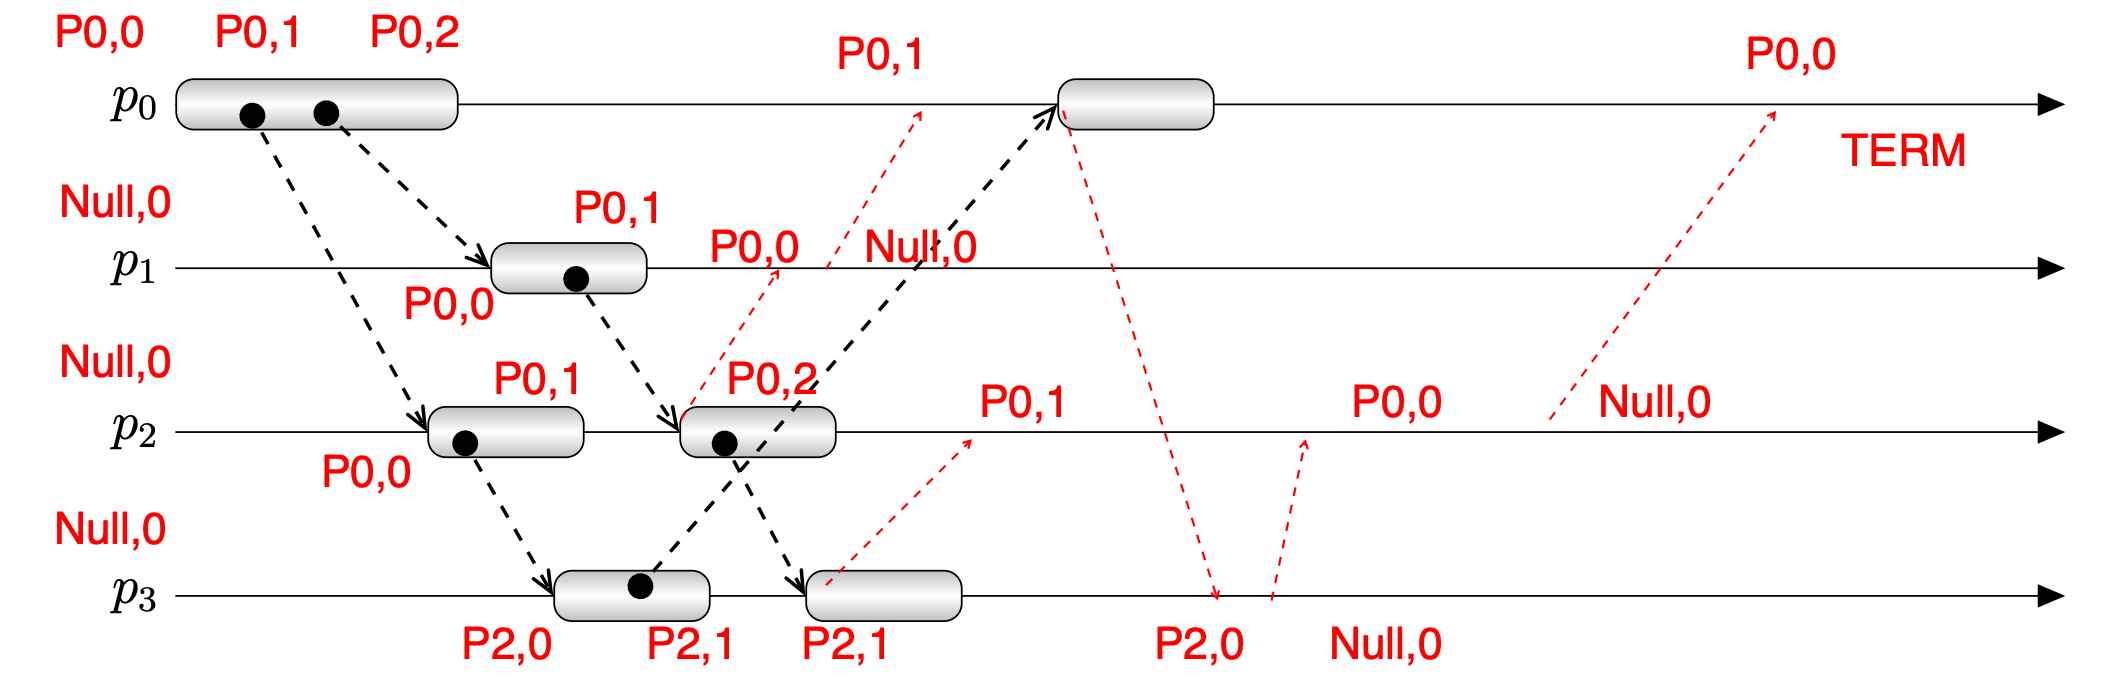
\includegraphics[width=\textwidth]{p1}
\subsection{Safra}
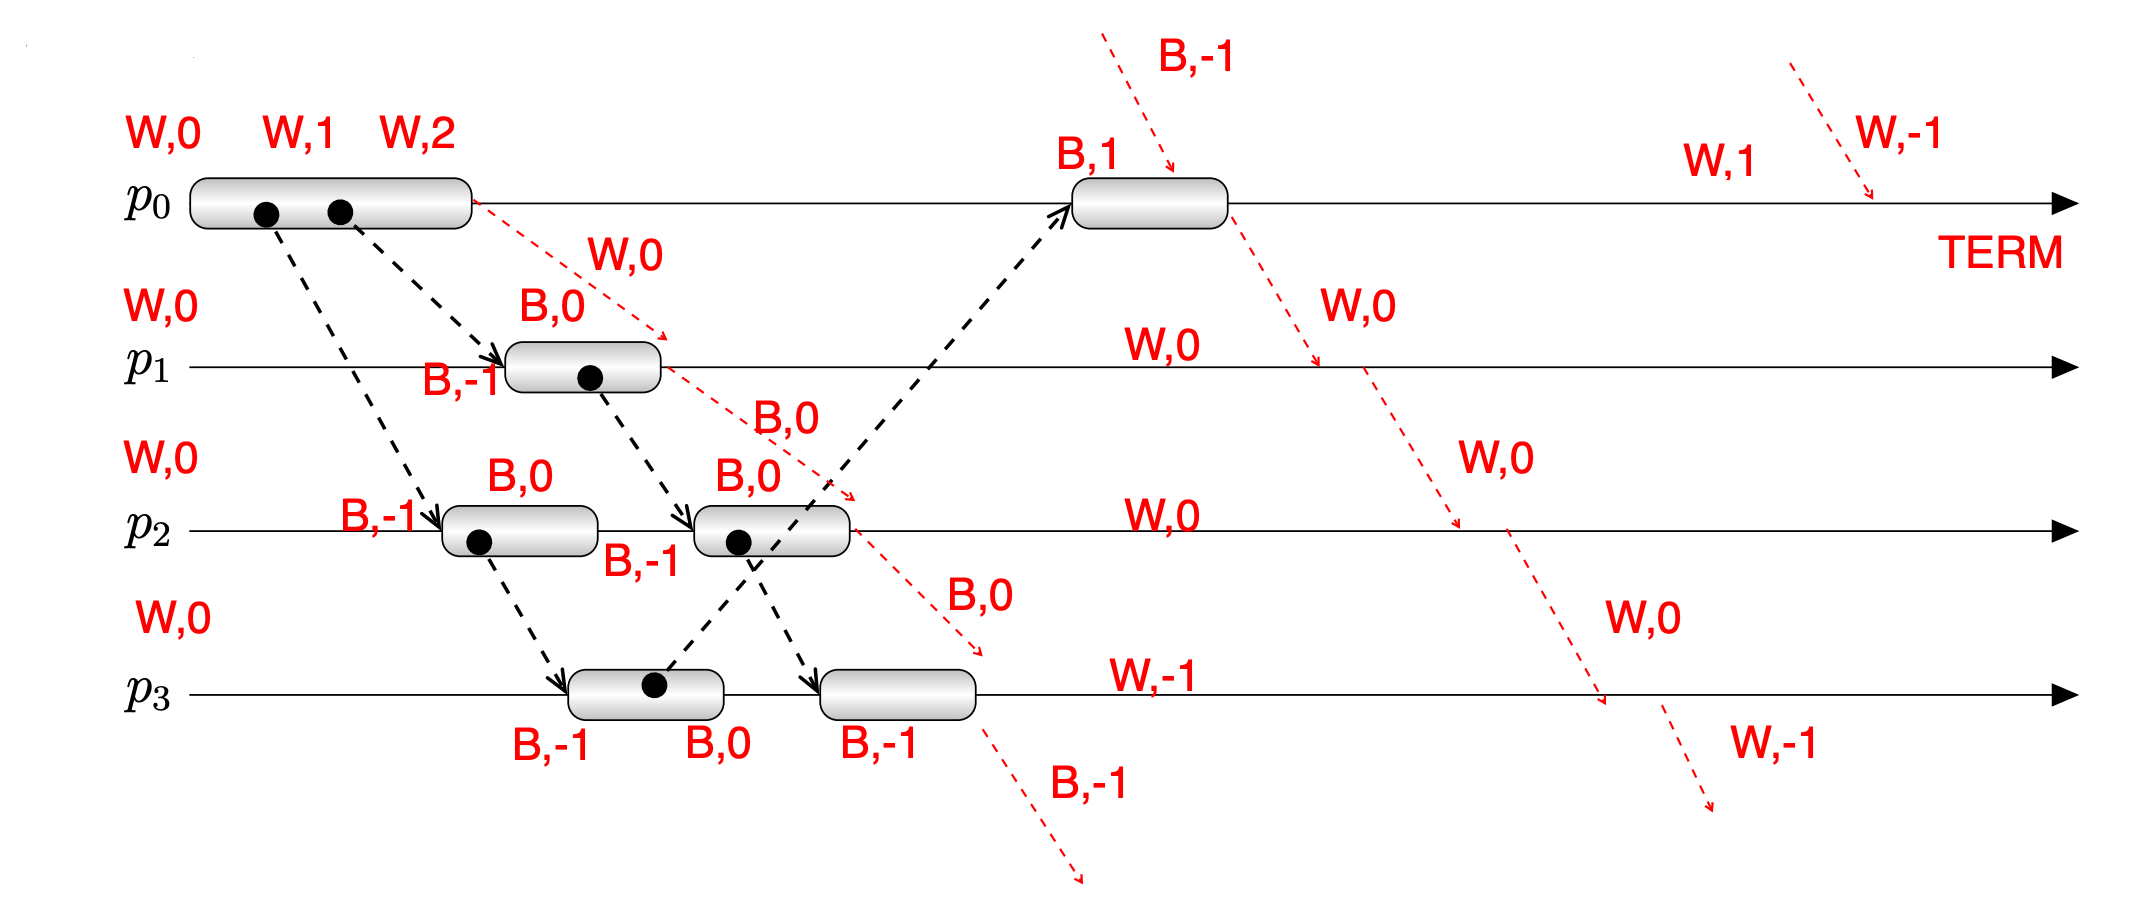
\includegraphics[width=\textwidth]{p2}

\section{Leader Election}

\subsection{Algorithm}

The basic idea is using Tarry's Traversal algorithm.
At first, we assume that the identity of no process is -1.
Every process will launch Tarry's Traversal algorithm with its own identity as token simultaneously.
If a process with a greater identity is reached, the traversal will stop earlier.
Furthermore, the greater process will send -1 as token back to its parent.
And the process will also send -1 back directly if it receives -1.
At last, the process can be leader if its identity goes back.

\begin{algorithm}[H]

  \fRecv{START()}{}{
    $done_i \gets false;$
    $elected_i \gets false;$

    \fSend{$k$}{$neighbors_i$}{GO($i, i, id_i$)}{$p_k$}
  }

  \fNewLine

  \fRecv{GO($root, pre, id_{root}$)}{}{
    \If{$id_{root} = -1$ or $id_{root} < id_i$}{
      \fSend{}{}{GO($root, i, -1$)}{$p_{pre}$}
    }
    \If{$parent_{i,root} = \perp$}{
      $parent_{i,root} \gets pre$\;
      $unreached_{i,root} \gets neighbors_i \backslash \{pre\};$
    }
    \eIf{$unreached_{i,root} \ne \emptyset$}{
      \tcc{pop() will return an element in the set then remove it from the set.}
      $next \gets pop(unreached_{i,root})$\;
      \fSend{}{}{GO($root, i, id_{root}$)}{$p_{next}$}
    }{
      \eIf{$i = parent_i$}{
        \If{$id_{root} != -1$}{
          $elected_i \gets true$
        }
        $done_i \gets true;$\;
        terminate()\;
      }{
      \fSend{}{}{GO($root, i, id_{root}$)}{$p_{parent_i}$}
      }
    }
  }

  \caption{Leader Election}
\end{algorithm}

\subsection{Safety}
\subsubsection{$elected_i$ and $done_i$ are locally stable predicates}
\begin{enumerate}
  \item Every process only starts one time.
  \item $elected_i$ and $done_i$ only be changed before terminate().
  \item $elected_i$ and $done_i$ only be changed once time.
  \item $elected_i$ and $done_i$ are locally stable predicates.
\end{enumerate}
Q.E.D.

\subsubsection{at most one process is leader (e.g., done and elected).}
\begin{enumerate}
  \item Every process launches the Leader Election algorithm.
  \item There is only one process with the greatest identity.
  \item Only one process's traversal can send the original identity back.
  \item Only one process can be leader.
\end{enumerate}
Q.E.D.

\subsubsection{a process cannot be done if no process is elected.}
\begin{enumerate}
  \item Every process launches the Leader Election algoirthm.
  \item The greatest process launches the Leader Election algorithm.
  \item Every process will terminate.
  \item The greatest process will be leader.
  \item After all the processes are completed, there will be a leader.
\end{enumerate}
Q.E.D.

\subsection{Liveness}

\subsubsection{after some time, a process is elected.}
\begin{enumerate}
  \item The greatest process launches the Leader Election algorithm.
  \item Its traversal will go through all other processes.
  \item Its identity will go back to iteself.
  \item Eventually the greatest process is leader.
\end{enumerate}
Q.E.D.

\subsubsection{after some tome, all processes are done.}
\begin{enumerate}
  \item The process will send -1 back to its parent if its identity is greater than the root's.
  \item The process will send -1 back to its parent if it receives -1.
  \item Otherwise, the process will go through all other neighbors.
  \item The $unreached_{i,root}$ will be empty. At that time, the process will return the root's identity.
  \item All the process will return to its parent.
  \item All the roots will be done.
\end{enumerate}
Q.E.D.

\end{document}
